%%%%%%%%%%%%%%%%%%%%%%%%%%%%%%%%%%%%%%%%%
% Arsclassica Article
% LaTeX Template
% Version 1.1 (1/8/17)
%
% This template has been downloaded from:
% http://www.LaTeXTemplates.com
%
% Original author:
% Lorenzo Pantieri (http://www.lorenzopantieri.net) with extensive modifications by:
% Vel (vel@latextemplates.com)
%
% License:
% CC BY-NC-SA 3.0 (http://creativecommons.org/licenses/by-nc-sa/3.0/)
%
%%%%%%%%%%%%%%%%%%%%%%%%%%%%%%%%%%%%%%%%%

%----------------------------------------------------------------------------------------
%	PACKAGES AND OTHER DOCUMENT CONFIGURATIONS
%----------------------------------------------------------------------------------------

\documentclass[
10pt, % Main document font size
a4paper, % Paper type, use 'letterpaper' for US Letter paper
oneside, % One page layout (no page indentation)
%twoside, % Two page layout (page indentation for binding and different headers)
headinclude,footinclude, % Extra spacing for the header and footer
BCOR5mm, % Binding correction
]{scrartcl}

%%%%%%%%%%%%%%%%%%%%%%%%%%%%%%%%%%%%%%%%%
% Arsclassica Article
% Structure Specification File
%
% This file has been downloaded from:
% http://www.LaTeXTemplates.com
%
% Original author:
% Lorenzo Pantieri (http://www.lorenzopantieri.net) with extensive modifications by:
% Vel (vel@latextemplates.com)
%
% License:
% CC BY-NC-SA 3.0 (http://creativecommons.org/licenses/by-nc-sa/3.0/)
%
%%%%%%%%%%%%%%%%%%%%%%%%%%%%%%%%%%%%%%%%%

%----------------------------------------------------------------------------------------
%	REQUIRED PACKAGES
%----------------------------------------------------------------------------------------

\usepackage[
nochapters, % Turn off chapters since this is an article        
beramono, % Use the Bera Mono font for monospaced text (\texttt)
eulermath,% Use the Euler font for mathematics
pdfspacing, % Makes use of pdftex’ letter spacing capabilities via the microtype package
dottedtoc % Dotted lines leading to the page numbers in the table of contents
]{classicthesis} % The layout is based on the Classic Thesis style

\usepackage{arsclassica} % Modifies the Classic Thesis package

\usepackage[T1]{fontenc} % Use 8-bit encoding that has 256 glyphs

\usepackage[utf8]{inputenc} % Required for including letters with accents

\usepackage{graphicx} % Required for including images
\graphicspath{{Figures/}} % Set the default folder for images

\usepackage{enumitem} % Required for manipulating the whitespace between and within lists

\usepackage{lipsum} % Used for inserting dummy 'Lorem ipsum' text into the template

\usepackage{subfig} % Required for creating figures with multiple parts (subfigures)

\usepackage{amsmath,amssymb,amsthm} % For including math equations, theorems, symbols, etc

\usepackage{varioref} % More descriptive referencing

%----------------------------------------------------------------------------------------
%	THEOREM STYLES
%---------------------------------------------------------------------------------------

\theoremstyle{definition} % Define theorem styles here based on the definition style (used for definitions and examples)
\newtheorem{definition}{Definition}

\theoremstyle{plain} % Define theorem styles here based on the plain style (used for theorems, lemmas, propositions)
\newtheorem{theorem}{Theorem}

\theoremstyle{remark} % Define theorem styles here based on the remark style (used for remarks and notes)

%----------------------------------------------------------------------------------------
%	HYPERLINKS
%---------------------------------------------------------------------------------------

\hypersetup{
%draft, % Uncomment to remove all links (useful for printing in black and white)
colorlinks=true, breaklinks=true, bookmarks=true,bookmarksnumbered,
urlcolor=webbrown, linkcolor=RoyalBlue, citecolor=webgreen, % Link colors
pdftitle={}, % PDF title
pdfauthor={\textcopyright}, % PDF Author
pdfsubject={}, % PDF Subject
pdfkeywords={}, % PDF Keywords
pdfcreator={pdfLaTeX}, % PDF Creator
pdfproducer={LaTeX with hyperref and ClassicThesis} % PDF producer
} % Include the structure.tex file which specified the document structure and layout

\hyphenation{Fortran hy-phen-ation} % Specify custom hyphenation points in words with dashes where you would like hyphenation to occur, or alternatively, don't put any dashes in a word to stop hyphenation altogether

%----------------------------------------------------------------------------------------
%	TITLE AND AUTHOR(S)
%----------------------------------------------------------------------------------------

\title{\normalfont{Study of Cold Nuclear Matter effect with prompt $D_s$ meson production in pPb collisions at LHCb}} % The article title

%\subtitle{Subtitle} % Uncomment to display a subtitle

\author{{Chenxi Gu}} % The article author(s) - author affiliations need to be specified in the AUTHOR AFFILIATIONS block

\date{} % An optional date to appear under the author(s)

%----------------------------------------------------------------------------------------

\begin{document}

%----------------------------------------------------------------------------------------
%	HEADERS
%----------------------------------------------------------------------------------------

\renewcommand{\sectionmark}[1]{\markright{\spacedlowsmallcaps{#1}}} % The header for all pages (oneside) or for even pages (twoside)
%\renewcommand{\subsectionmark}[1]{\markright{\thesubsection~#1}} % Uncomment when using the twoside option - this modifies the header on odd pages
\lehead{\mbox{\llap{\small\thepage\kern1em\color{halfgray} \vline}\color{halfgray}\hspace{0.5em}\rightmark\hfil}} % The header style

\pagestyle{scrheadings} % Enable the headers specified in this block

%----------------------------------------------------------------------------------------
%	TABLE OF CONTENTS & LISTS OF FIGURES AND TABLES
%----------------------------------------------------------------------------------------

\maketitle % Print the title/author/date block

\setcounter{tocdepth}{2} % Set the depth of the table of contents to show sections and subsections only

\tableofcontents % Print the table of contents

\listoffigures % Print the list of figures

\listoftables % Print the list of tables

%----------------------------------------------------------------------------------------
%	ABSTRACT
%----------------------------------------------------------------------------------------

\section*{Abstract} % This section will not appear in the table of contents due to the star (\section*)

The productions of prompt $D_s$ mesons in proton-lead collisions in the forward and backward configurations are studied. The data are collected with the LHCb detector with $\sqrt{s_{NN}} = 5TeV$(proton beam energy is 4000 GeV,lead beam energy is 1500 GeV). The forward (backward) rapidity range $1.5<y^*<3.5(-4.5<y^*<-2.5)$, the $p_T$ range $0<p_T<10GeV/c$. The paper will introduce my work this semaster. % Dummy text

%----------------------------------------------------------------------------------------
%	AUTHOR AFFILIATIONS
%----------------------------------------------------------------------------------------

%----------------------------------------------------------------------------------------

\newpage % Start the article content on the second page, remove this if you have a longer abstract that goes onto the second page

%----------------------------------------------------------------------------------------
%	INTRODUCTION
%----------------------------------------------------------------------------------------

\section{Introduction}

Ultra-relativistic heavy-ion collisions are used to study the nuclear matter at high temperature and pressure where the formation of the Quark Gluon Plasma (QGP), a state of matter which consists of asymptotically free quarks and gluons, occurs. Open heavy flavours and quarkonia are produced at the early stages of the collision and might interact with the deconfined medium, making them ideal probes of the QGP. It was indeed predicted that in hot nuclear matter, charmonia are suppressed due to color screening of the heavy quarks potential . Quarkonia can also be suppressed in absence of the QGP formation by Cold Nuclear Matter (CNM) effects. Proton-Nucleus collisions (pA or Ap), which are interesting by themselves, are therefore essential to interpret Nucleus-Nucleus data in order to disentangle QGP effects from CNM effects in those collisions. The main CNM effects affecting quarkonium production include initial-state nuclear effects on the parton densities , the initial-state parton energy loss and final-state energy loss , the final- state absorption of the pre-resonant heavy quark pair by the spectator nucleons  albeit small at LHC  and the final-state interaction of the quarkonium with the produced medium .
 %----------------------------------------------------------------------------------------
%	METHODS
%----------------------------------------------------------------------------------------

\section{LHCb advantage in heavy ion physics}


\begin{itemize}[noitemsep] % [noitemsep] removes whitespace between the items for a compact look
\item LHCb is specialised in heavy flavour precision physics, beauty and charm:
\begin{itemize}
\item Optimised for low pile-up collisions(ie low multiplicity):
\begin{itemize}
\item Precise reconstruction of production and decay vertices: time dependent CP violation
\item Correlations between particles: flavour tagging
\end{itemize}
\end{itemize}
\item Some characteristics of the experiment make it attractive for measurements in Heavy ion physics too:
\begin{itemize}
\item Instruments fully the forward region:$2<\eta<5$
\item Precise vertexing:separation of prompt production from B decay products
\item Precise tracking:reconstruction down to $p_T=0$
\item Particle identification:full reconstruction of hadronic decays of charm or beauty, such as $D_0 \rightarrow K\pi $
\end{itemize}
\end{itemize}

%------------------------------------------------
%----------------------------------------------------------------------------------------
%	Cross-section determination
%----------------------------------------------------------------------------------------
\section{Cross-section Determination}
    The determination of the double-differential production cross-section for prompt $D_s$ requires the knowledge of the numbers of prompt $D_s$ in bins of the kinematic variables4 $y^{*}$ and $p_{T}$, where $p_T$ and $y^{*}$ are defined in the nucleon-nucleon center-of-mass frame, and the positive z-axis is defined as the direction of the proton beam.\par
    The laboratory frame does not coincide with the center-of-mass frame of the proton-nucleon system, which has a rapidity of $\delta y = \frac
{1}{2} log(A_{Pb}/Z_{Pb}) = 0.465$ in the laboratory frame. Therefore the rapidity in the pN rest frame, $y^{*}$, is shifted by a constant value with respect to the rapidity in the laboratory frame, $y = y^{*} + 0.465$.\par
Here we define the rapidity with the direction of proton beam as positive z-axis (lead beam as negative z-axis). We thus define the rapidity acceptance in the pN center-of-mass frame to be$1.5<y^{*} <3.5(-4.5<y^{*} <-2.5)$for the Fwd(Bwd) collision. For the differential cross-section determination, the bin width for $p_T$ is 1 GeV/c and for $y^{*}$ 0.5; the signal yields and efficiency are determined separately for each bin, thanks to the good resolution.
The double differential cross-section for prompt $D_s$ production in a given $(p_T,y^{*})$ bin is thus defined as:
\begin{equation}
\frac{d^2\sigma}{dp_Tdy}=\frac{N(D_s\rightarrow K^+K^-\pi)}{L\times \epsilon_{tot}\times B(D_s\rightarrow K^+K^-\pi)\times \Delta y\times \Delta p_T}
\end{equation}
where
\begin{itemize}
\item $N(D_s\rightarrow K^+K^-\pi)$ is the number of prompt $D_s$ signals reconstructed through the $D_s\rightarrow K^+K^-\pi$ decay channel.
\item L is the integrated luminosity.
\item $\epsilon_{tot}$ is the total efficiency determined in each ($p_T,y^{*}$) bin
\item $B(D_s\rightarrow K^+K^-\pi)$  is the branching fraction of the decay $D_s^+\rightarrow K^+K^-\pi^+$ including $D_s^-\rightarrow K^+K^-\pi^-$
\item $\Delta p_T = 1$ GeV/c is the bin width of the $D_s$ transverse momentum.
\item $\Delta y = 0.5$ is the bin width of the $D_s$ rapidity.
\end{itemize}


The forward and backward cross-section measurements are in the range $p_T(D_s) <
 10$ GeV/c. The rapidity acceptance in the laboratory frame for $D_s$ is roughly $2 < y < 4$
 for the Fwd collision, and $-4 < y < -2$ for the Bwd collision.\par
 
 
The total cross-section over a specific range is determined by integrating the double differential cross-section over that particular range. The nuclear modification factor is defined to be the production cross-section in pPb collisions, normalized by the number of nucleons in Pb nucleus , relative to that in pp collisions corresponding to the same nucleon-nucleon center-of-mass energy $\sqrt{s_{NN}}$ ,

\begin{equation}
R_{pPb}=\frac{1}{A}\frac{\frac{d^2\sigma_{pPb}}{dp_Tdy^*}(y^*(p_T),\sqrt{s_{NN}})}{\frac{d^2\sigma_{pp}}{dp_Tdy^*}(y^*(p_T),\sqrt{s_{NN}})}
\end{equation}

studied in bins of $p_T$ and $y^*$ integrated over $y^*$ and $p_T$ respectively. As you can see,$R_{pPb}$ is calculated integrated in all centralities, i.e. averaged over the number of binary proton-nucleon collisions, which is estimated to be around 7 by the ALICE experiment at LHC . Another interesting variable is the forward-backward production ratio for the same absolute rapidity, defined as


\begin{equation}
R_{FB}=\frac{R_{pPb}(+|y^*|(p_T))}{R_{pPb}(-|y^*|(p_T))}
\end{equation}

also studied in bins of $p_T$ and $y^*$ integrated over $y^*$ and $p_T$ respectively.
%----------------------------------------------------------------------------------------
%	Signal yield determination
%----------------------------------------------------------------------------------------

\section{Signal yield determination}

The signal yield is determined from extended unbinned maximum likelihood fit to the $M(K^+K^-\pi)$ invariant mass distribution.The signal shape is described by a crystal ball function plus a Gaussian. The two components share the mean value $\mu$. In the CB function, we fix $n = 1$ constraint from physics, while a is fixed to 2.72, the value obtained from simulation. The fraction of the CB component is fixed to 0.76. These parameters are also obtained from simulation, and they are found to describe very well the simulation sample in different kinematic bins. The background is described by a linear function. We fit the candidates in the range $M \pm |\Delta M|$ around the observed $D_s$ mass as $M =1969$ MeV/c2, with $|\Delta M| = 79$ MeV/c2. In Fig. 1, the fitted signal yield in different $(p_T,y^*)$ bins are given. The $\sigma$ of the CB is known to depend on $D_s$ kinematics while the $\mu$ could also be kinematic dependent due to imperfect detector alignment, so in the fit the mean $\mu$ and $\sigma$ are independent parameters in each bin.\par

\begin{figure}[tb]
\centering
\subfloat[]{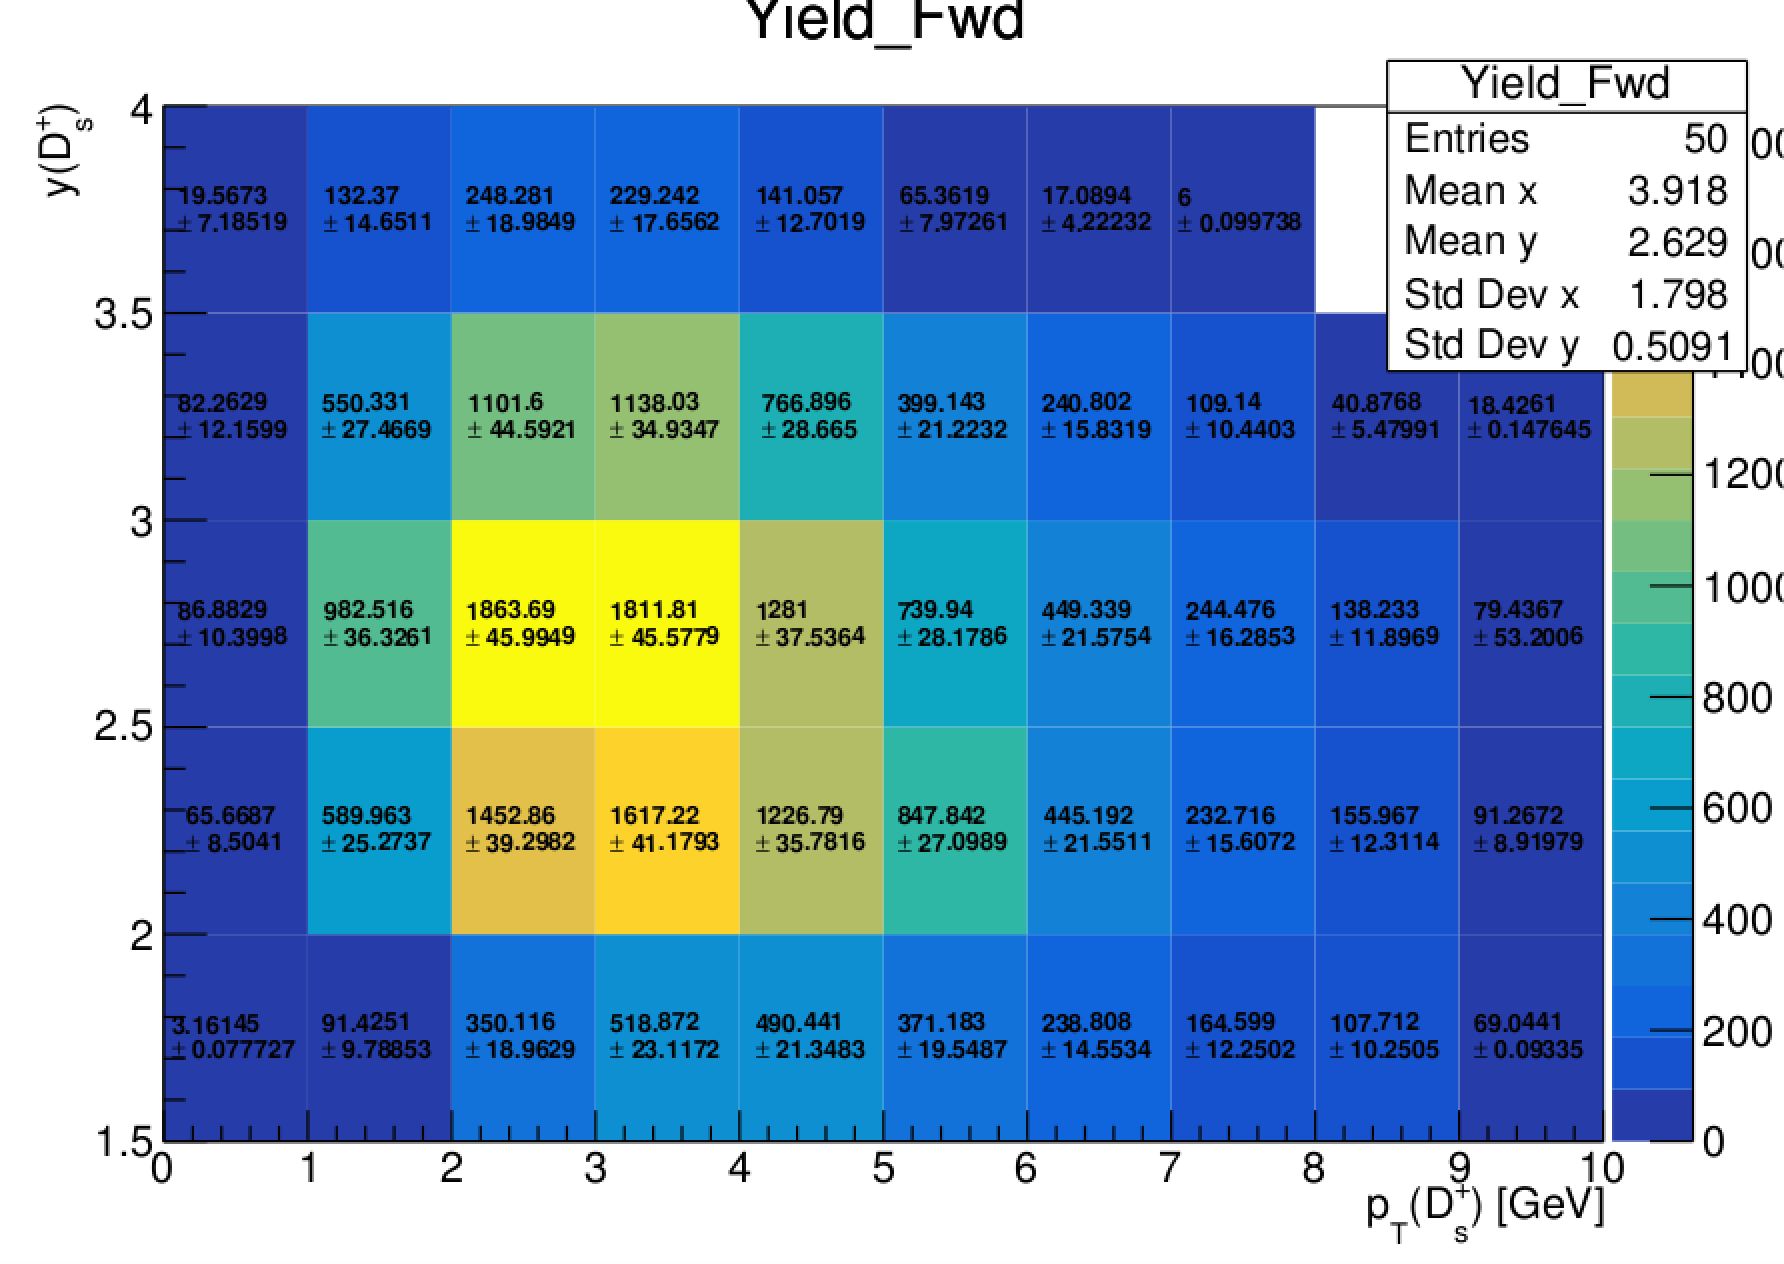
\includegraphics[width=.45\columnwidth]{Yield_pA}} \quad
\subfloat[]{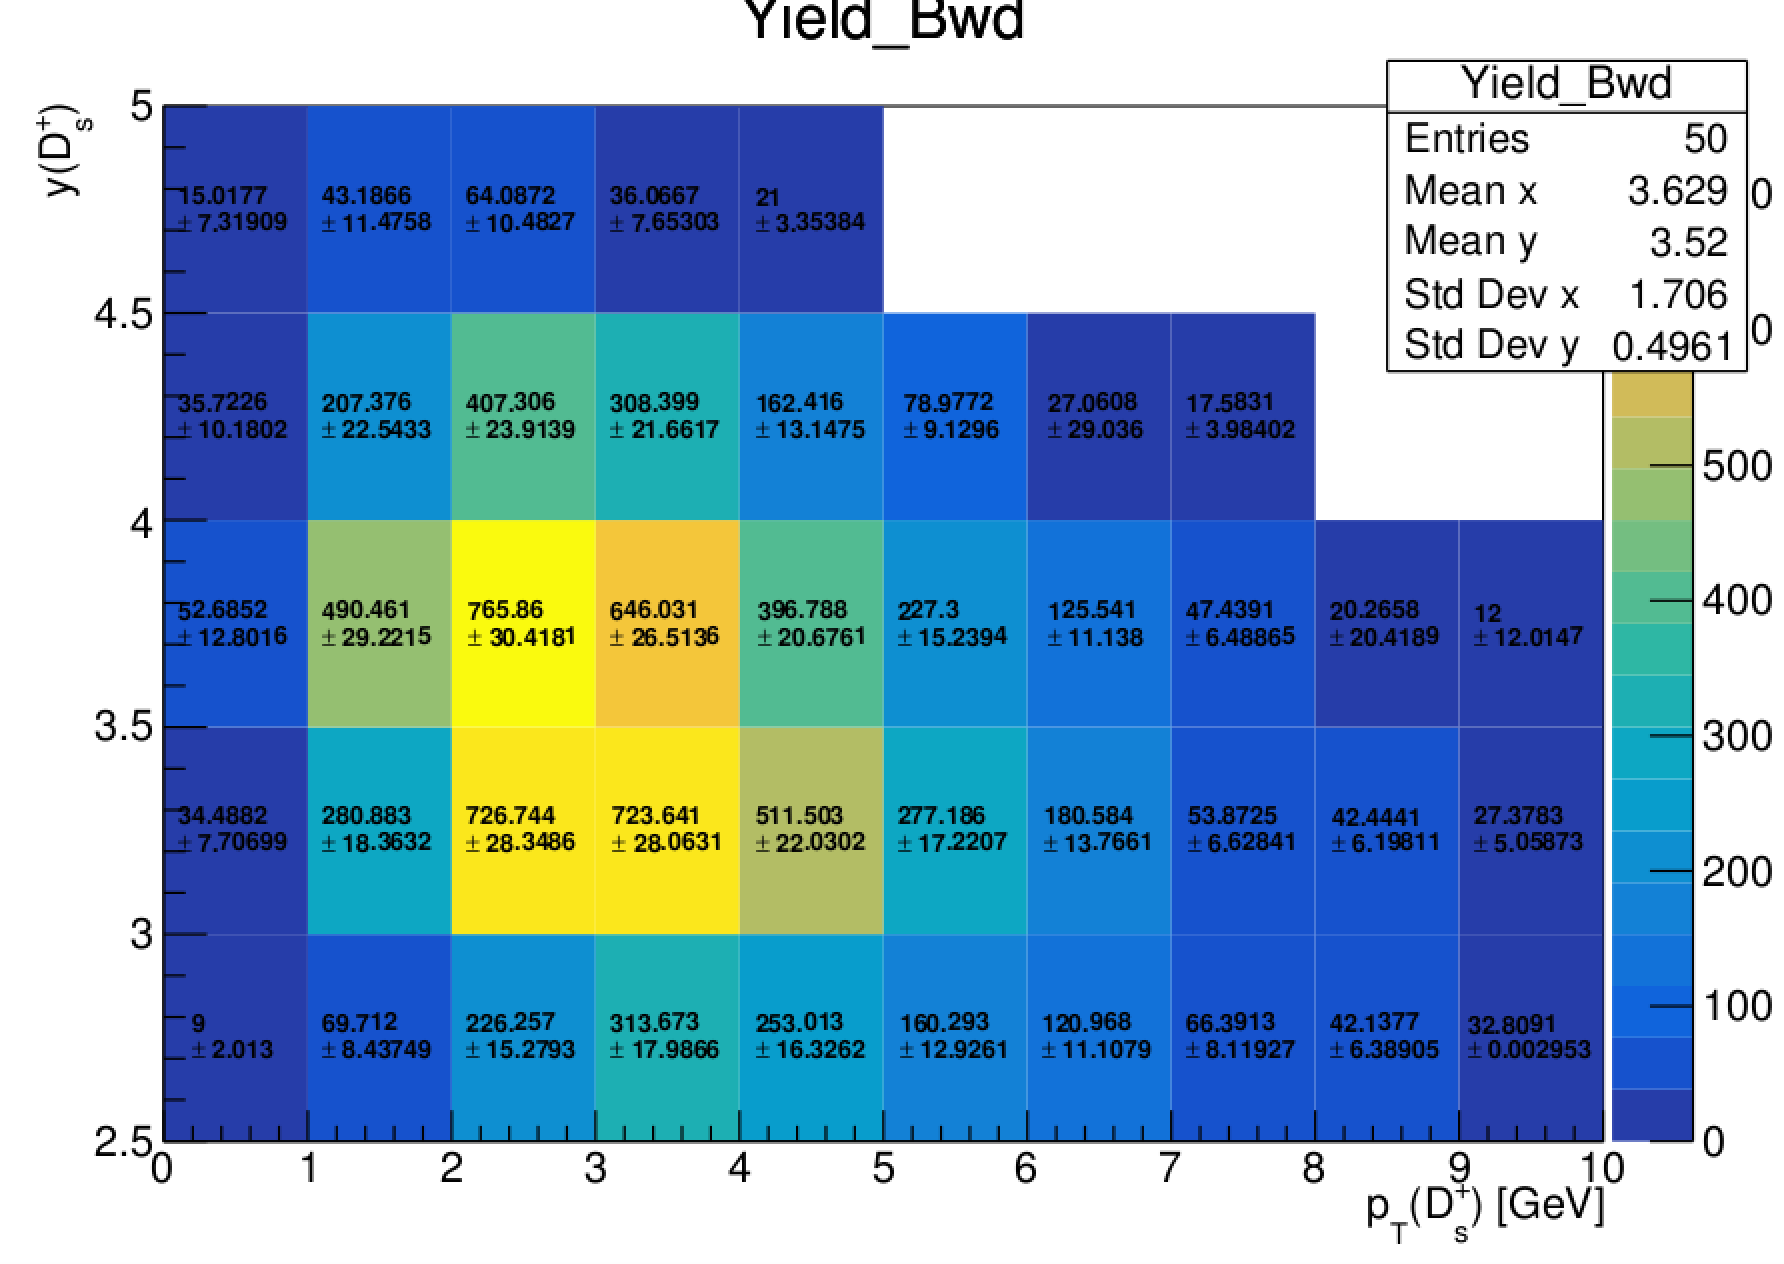
\includegraphics[width=.45\columnwidth]{Yield_Ap}} \quad
\caption[Signal yield]{The fitted total $D_s$ signal yields as a function of $p_T$ and $y^*$ for (left) Fwd and (right) Bwd real data configuration. The empty bins are regions in which the statistics was too low and the fit failed.} % The text in the square bracket is the caption for the list of figures while the text in the curly brackets is the figure caption
\label{fig:esempio}
\end{figure}


To discriminate prompt $D_s$ and $D_s$ from b, the distribution of $log(\chi^2_{IP}(D_s))$ (10 based logarithm) is fitted to determine the fraction of $D_s$ from b, which is the number of $D_s$ from b candidates over the sum of $D_s$ from b and prompt $D_s$. The $log(\chi^2_{IP}(D_s))$ for prompt $D_s$ decays is modelled with a modified gaussian function ($f_{AGE}$), where the width is allowed to be asymmetric with respect to the mean, and the tails are described by exponential functions


\begin{equation}
f_{AGE}(x;\mu,\sigma,\epsilon,\rho_L,\rho_R)=\left\{
\begin{aligned}
e^{\frac{\rho_L^2}{2}+\frac{\rho_L\cdot (x-\mu)}{\sigma \cdot (1-\epsilon)}} \quad\quad {x<\mu-(\sigma \cdot \rho_L\cdot(1-\epsilon))}\\
e^{-(\frac{x-\mu}{\sqrt{2}\sigma \cdot (1-\epsilon)})^2} \quad\quad {\mu-(\sigma \cdot \rho_L\cdot(1-\epsilon))<x<\mu}\\
e^{-(\frac{x-\mu}{\sqrt{2}\sigma \cdot (1+\epsilon)})^2} \quad\quad \mu <x<\mu+(\sigma \cdot \rho_R\cdot(1+\epsilon))\\
e^{\frac{\rho_R^2}{2}-\frac{\rho_R\cdot (x-\mu)}{\sigma \cdot (1+\epsilon)}} \quad\quad {x>\mu+(\sigma \cdot \rho_R\cdot(1+\epsilon))}\\
\end{aligned}
\right.
\end{equation}

as it was done in previous analyses The tail parameters $\rho_L$, $\rho_R$ and the asymmetry parameter $\epsilon$ are determined from fits to simulated sample.\par

The $log(\chi^2_{IP}(D_s))$ distribution for $D_s$-from-b component is described by a Gaussian function, while the one for combinatorial background is deduced by the S-weight method.\par

The fitted fractions in different $D_s$ $p_T$ and $y^*$ bins are given in Figs. 2. From the plot we can observe that the fraction lies in the range 0-0.2, and it increases with increasing $p_T$. It should be noted that these fractions should not be used to extract the production cross section of b-hadrons from that of $D_s$ production. In fact, the two components have very different efficiencies, in particular the lifetime-related selections favors b-hadrons.\par

The invariant mass and $log(\chi^2_{IP}(D_s))$ distributions, together with the fits are given in Figs. 3  for two particular kinematic bins, for the Fwd and Bwd sample respectively. Good agreements are found between the mass and $log(\chi^2_{IP}(D0))$ distributions of signals in data and simulation. 

\begin{figure}[tb]
\centering
\subfloat[]{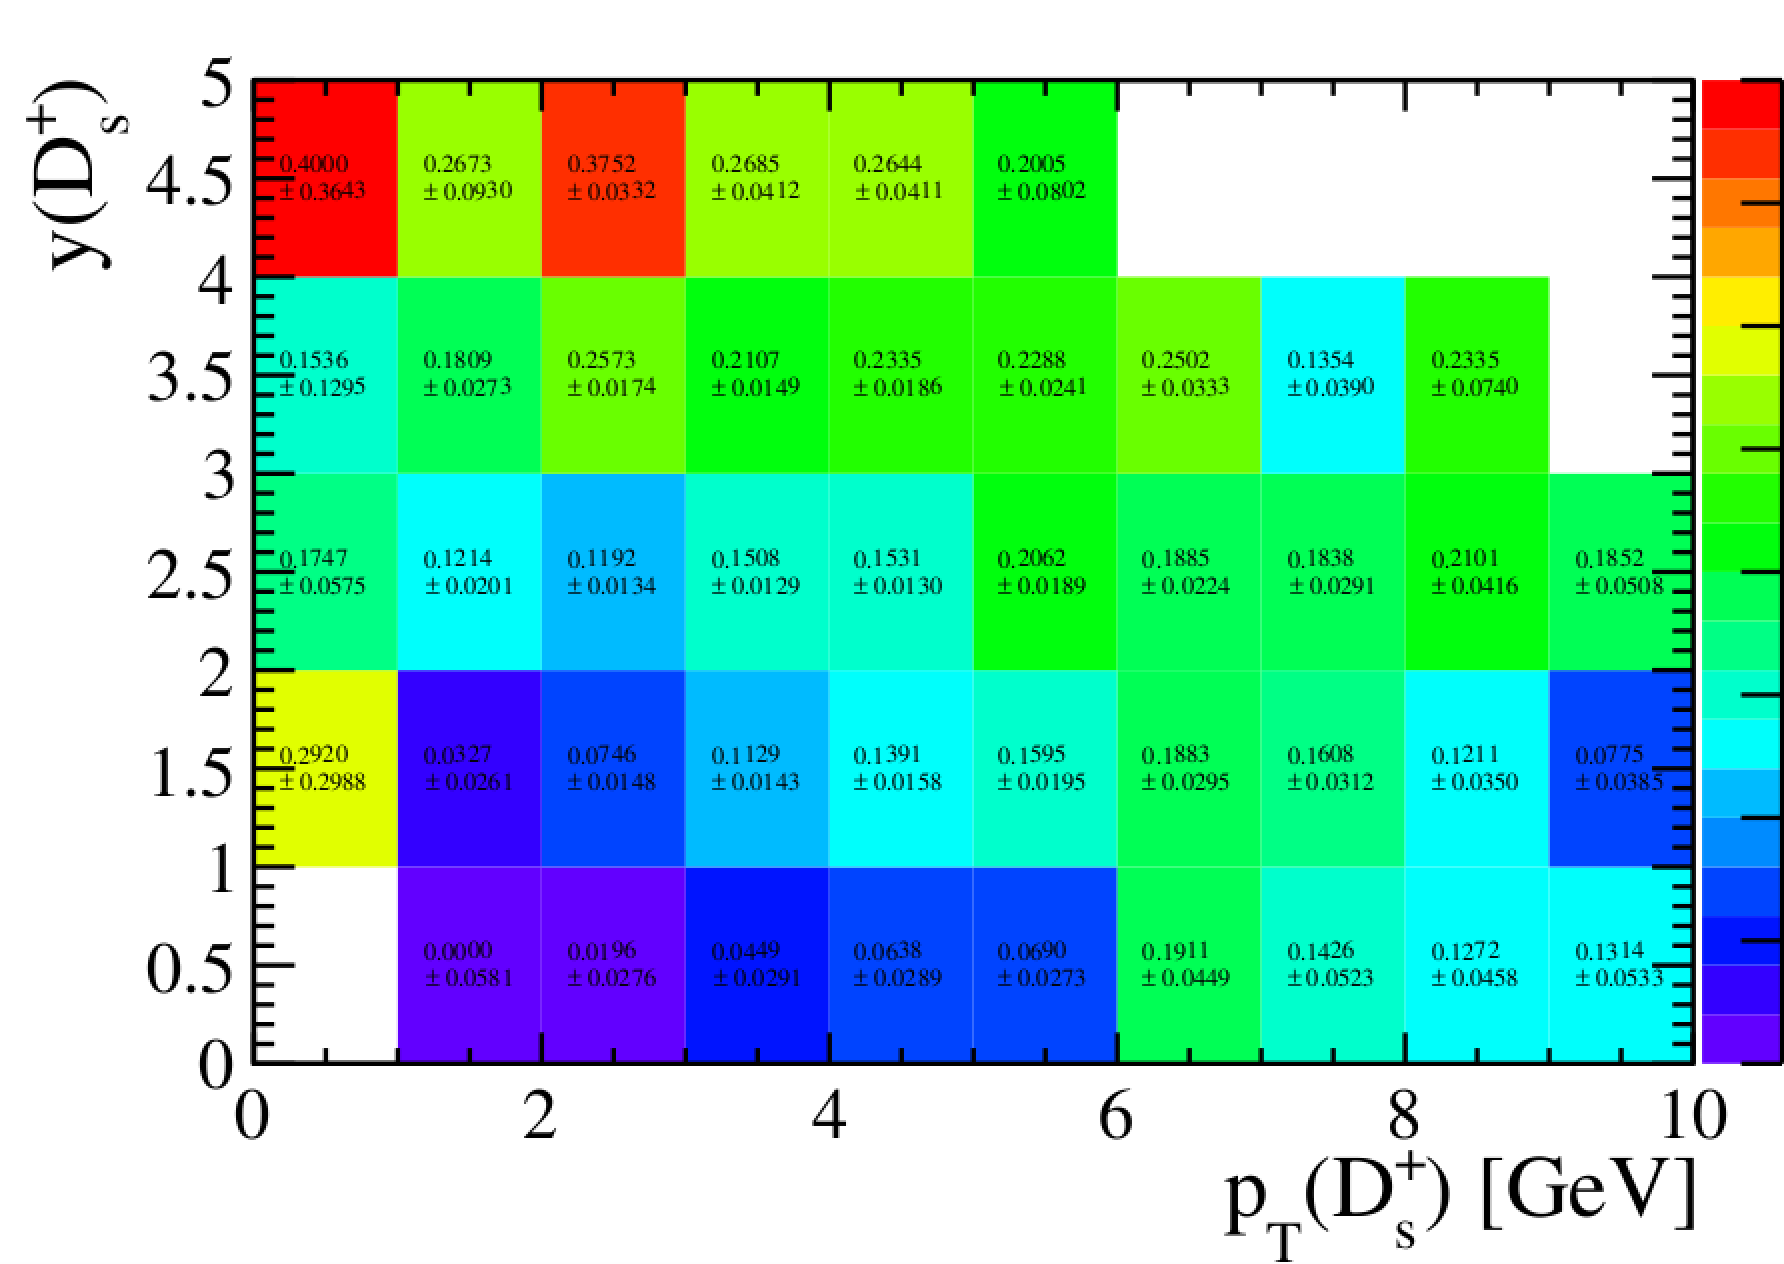
\includegraphics[width=.45\columnwidth]{BFraction_pA}} \quad
\subfloat[]{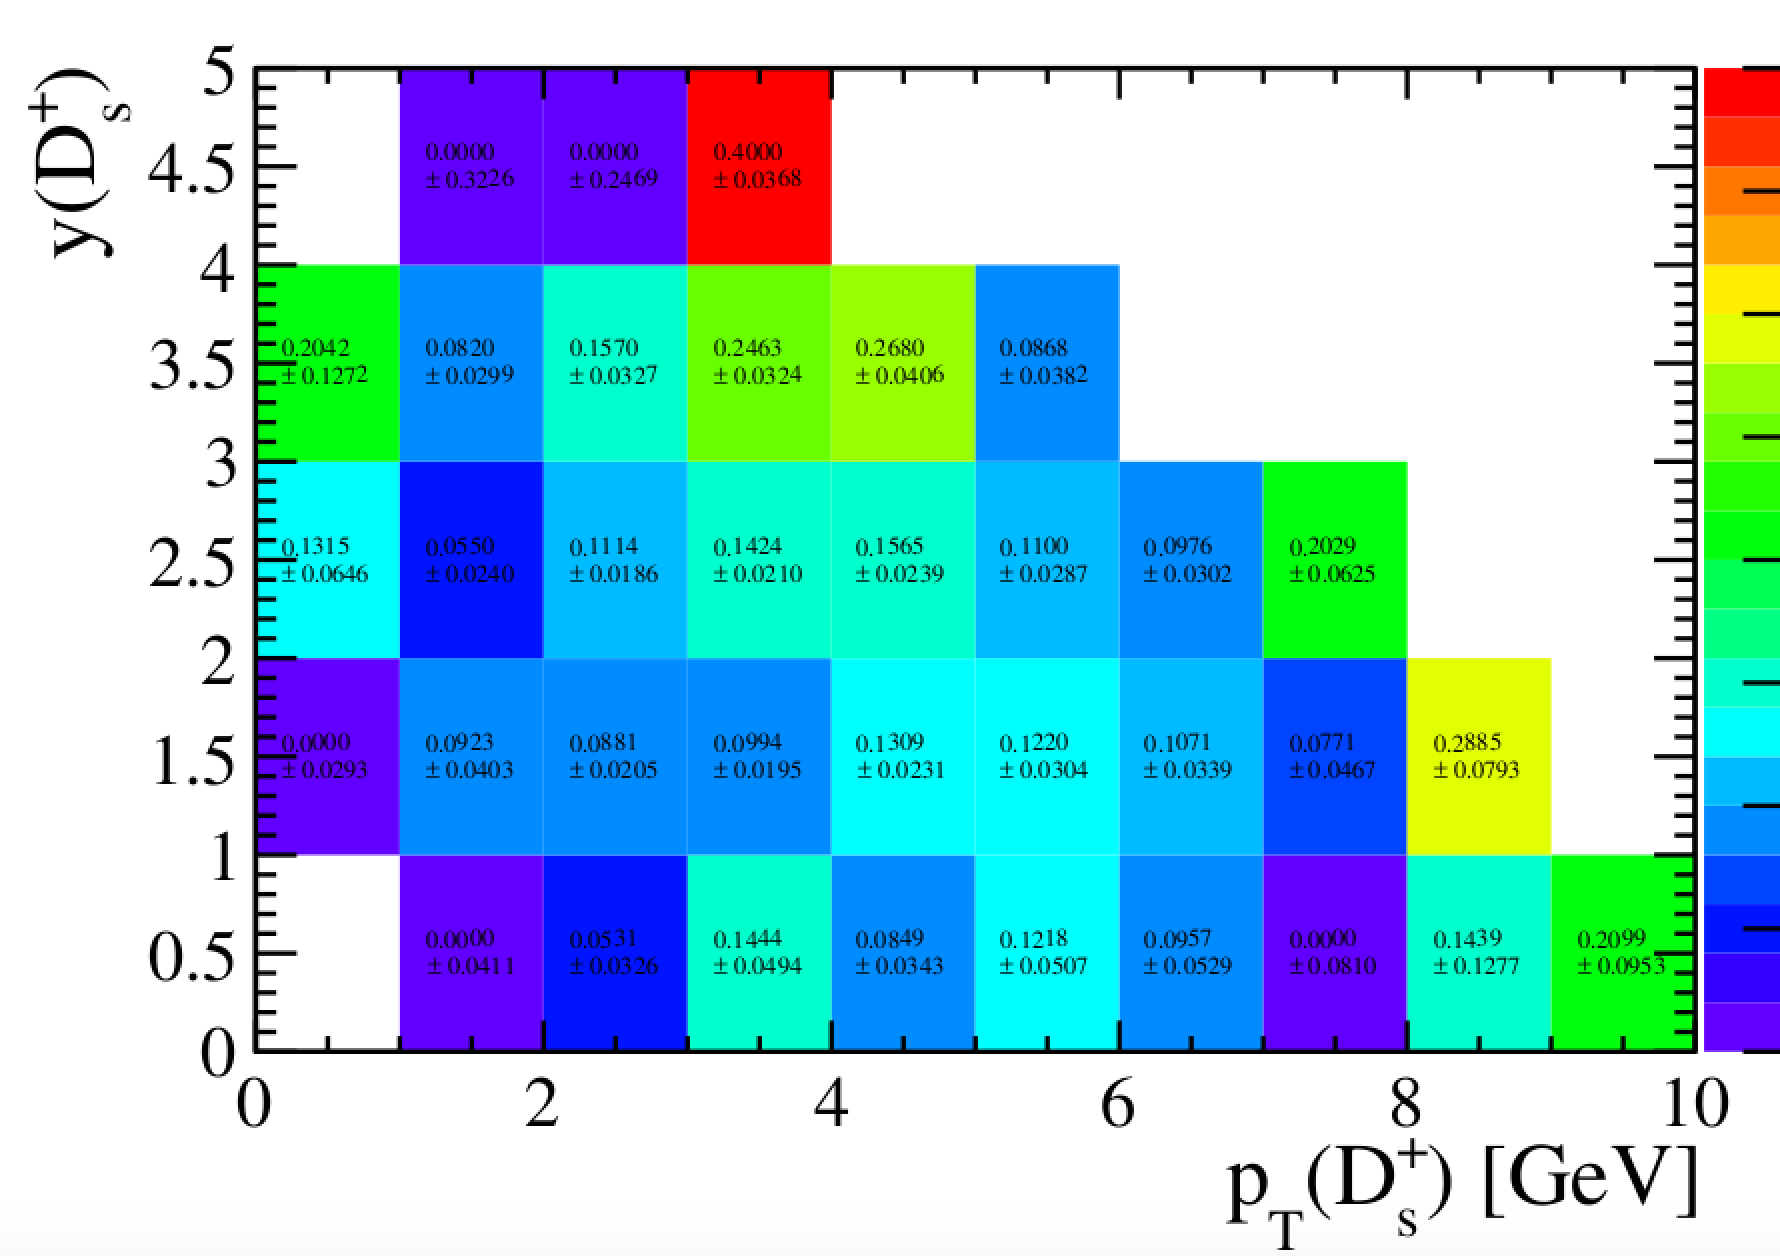
\includegraphics[width=.45\columnwidth]{BFraction_Ap}} \quad
\caption[$D_s$-from-b fraction]{The fitted fractions of $D_s$-from-b as a function of $p_T$ and $y^*$ for (left) Fwd and (right) Bwd data configuration. Only uncertainties returned by the fit are shown.} % The text in the square bracket is the caption for the list of figures while the text in the curly brackets is the figure caption
\label{fig:esempio}
\end{figure}



\begin{comment}
\begin{description}
\item[Word] Definition
\item[Concept] Explanation
\item[Idea] Text
\end{description}



\begin{itemize}[noitemsep] % [noitemsep] removes whitespace between the items for a compact look
\item First item in a list
\item Second item in a list
\item Third item in a list
\end{itemize}



\begin{table}[hbt]
\caption{Table of Grades}
\centering
\begin{tabular}{llr}
\toprule
\multicolumn{2}{c}{Name} \\
\cmidrule(r){1-2}
First name & Last Name & Grade \\
\midrule
 &  & $7.5$ \\
 &  & $2$ \\
\bottomrule
\end{tabular}
\label{tab:label}
\end{table}

Reference to Table~\vref{tab:label}. % The \vref command specifies the location of the reference
\end{comment}
%------------------------------------------------



\begin{figure}[tb]
\centering
\subfloat[]{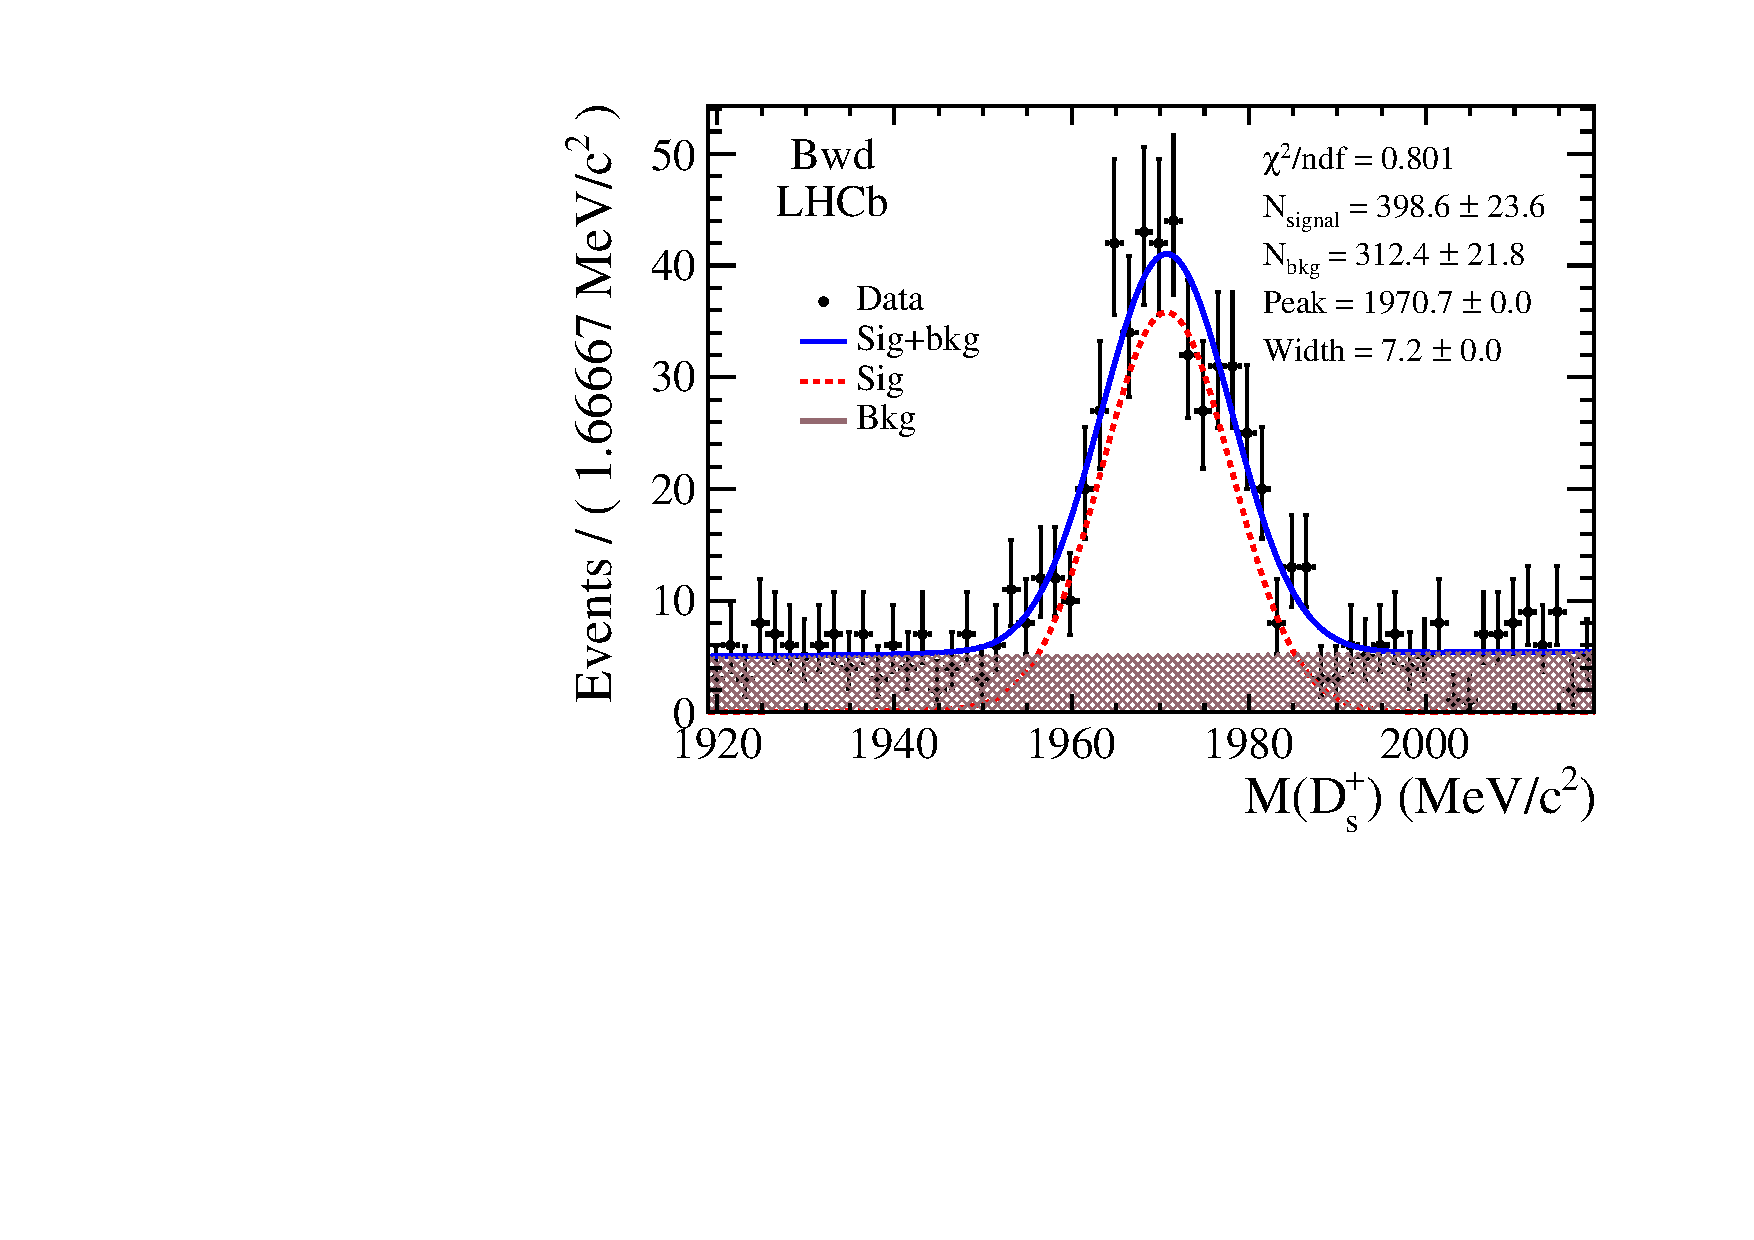
\includegraphics[width=.45\columnwidth]{Mass_Ap_2_3}} \quad
\subfloat[]{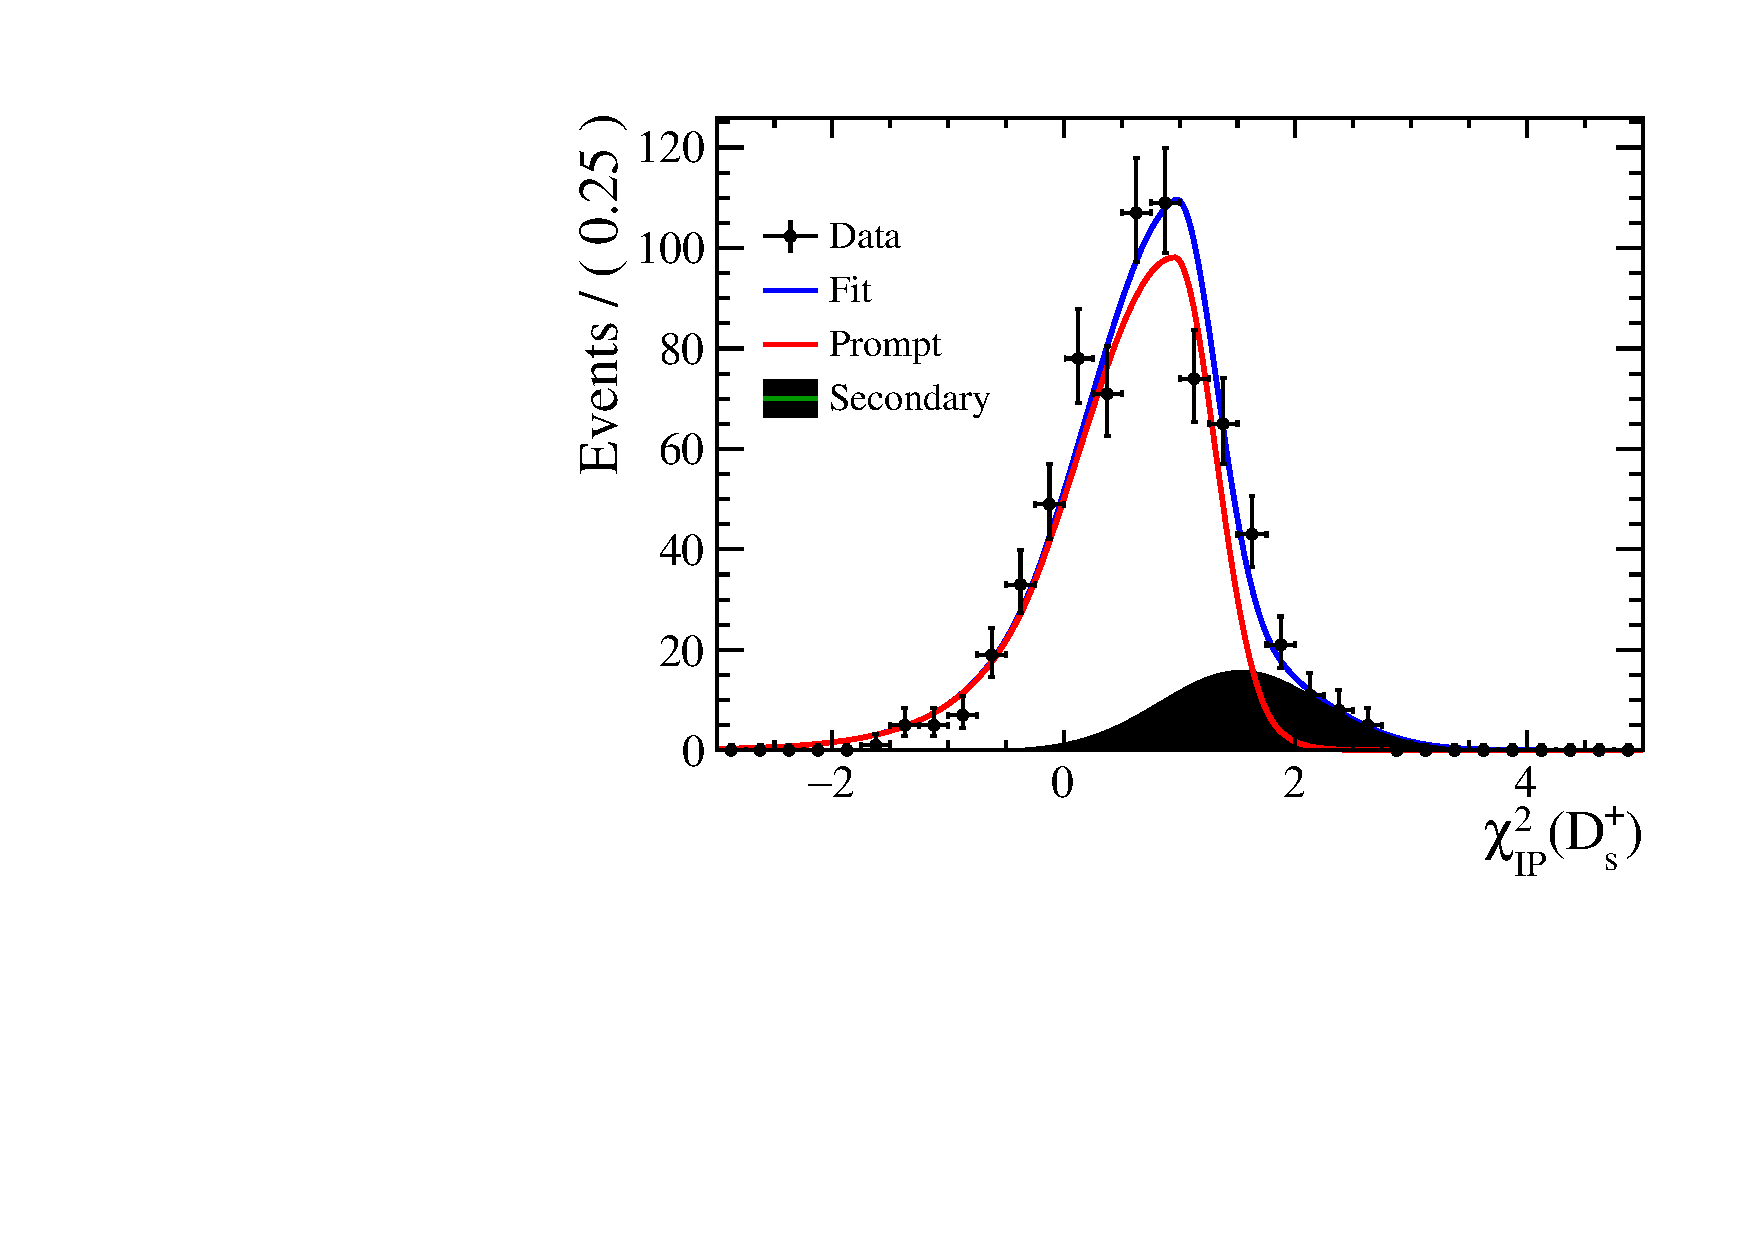
\includegraphics[width=.45\columnwidth]{IPCHI2_Ap_2_3}\label{IPCHI2_Ap_2_3}} \\
\subfloat[]{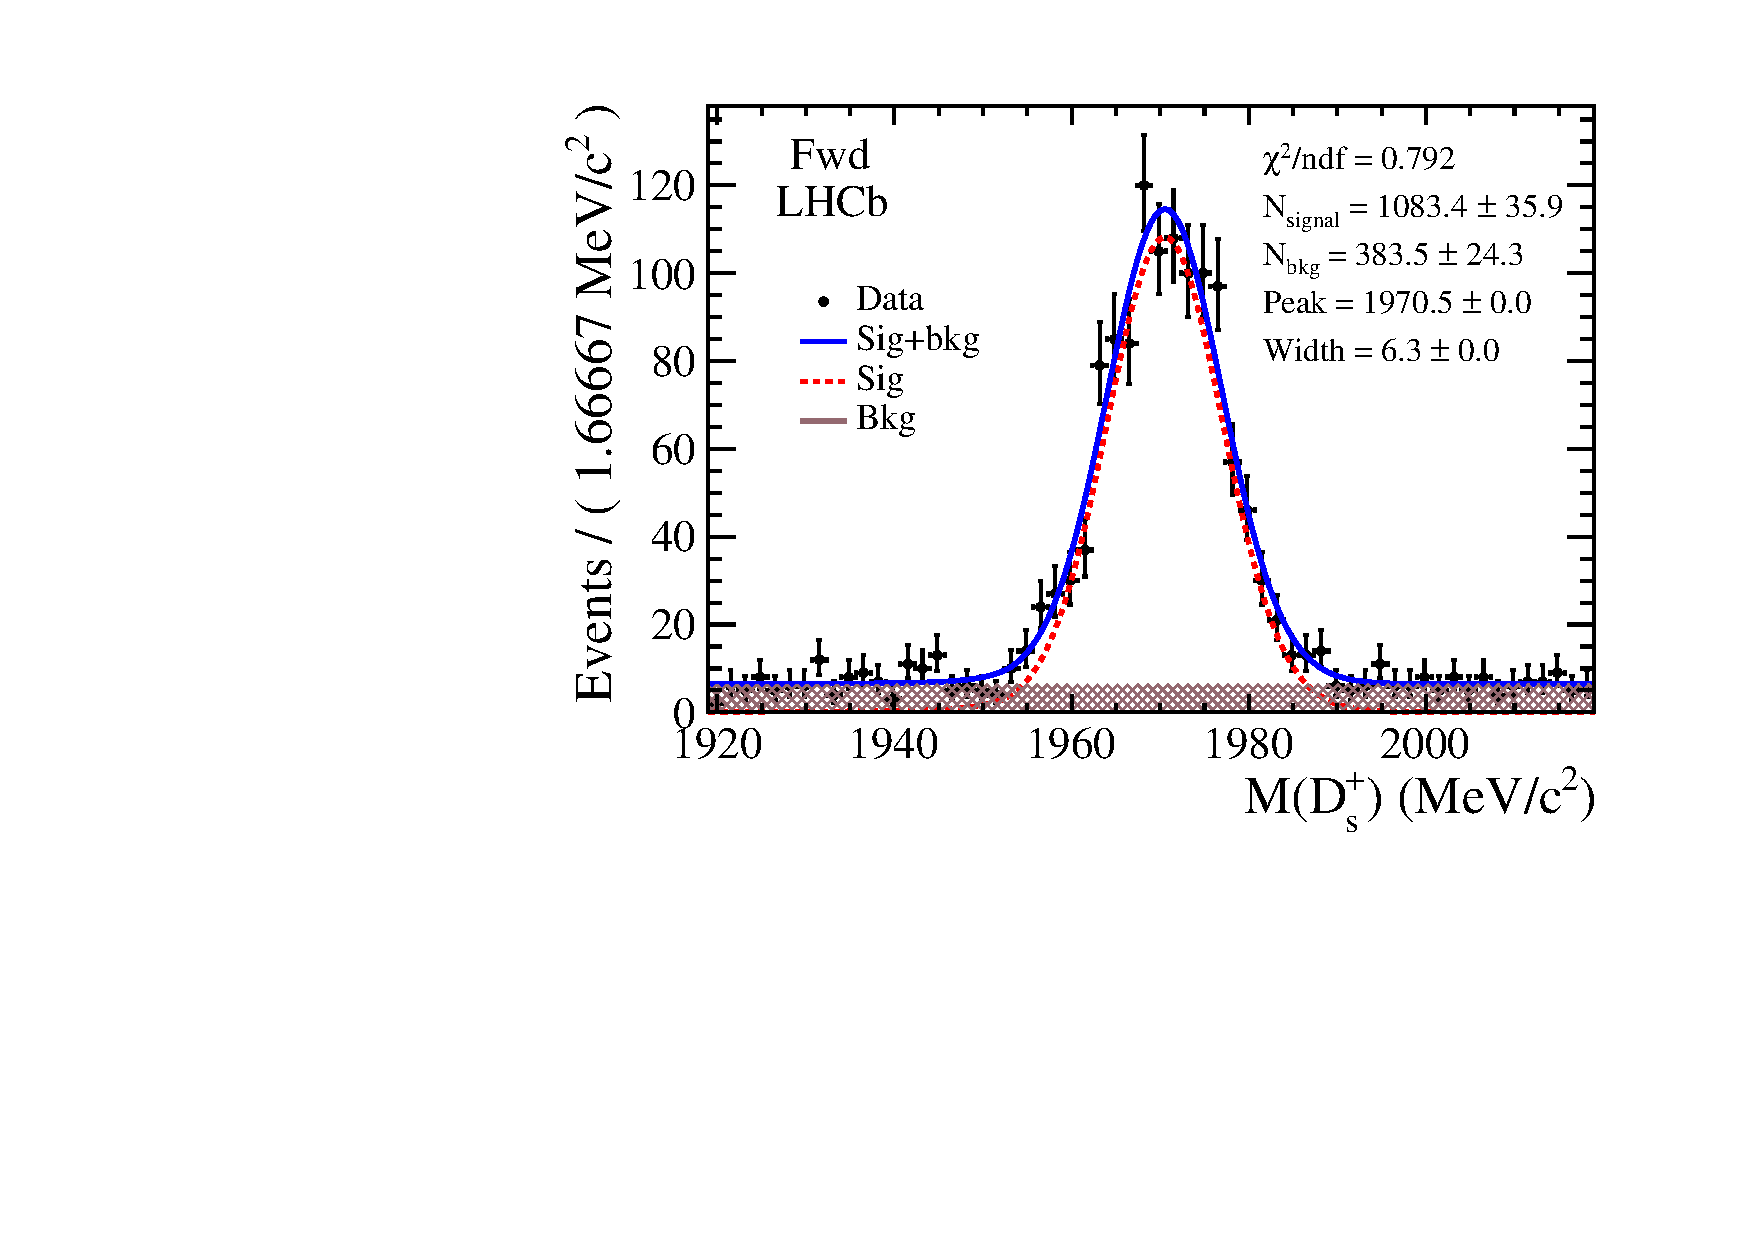
\includegraphics[width=.45\columnwidth]{Mass_pA_2_3}} \quad
\subfloat[]{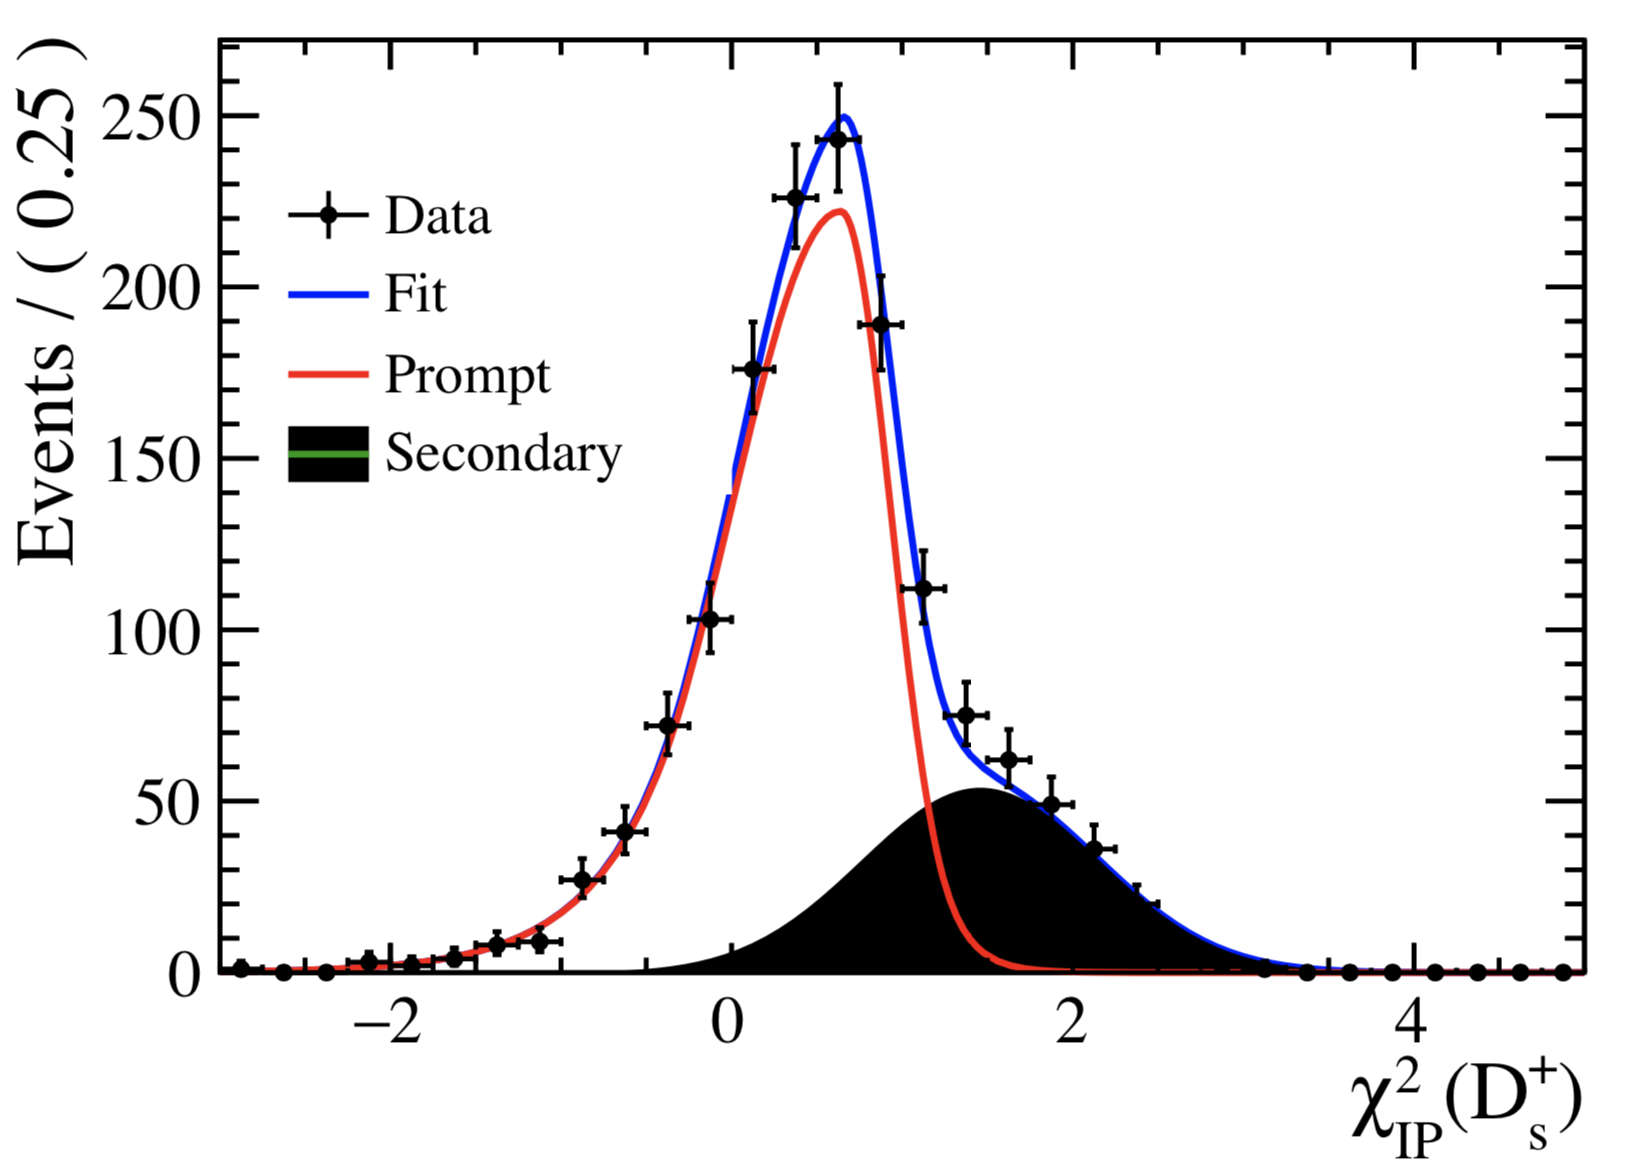
\includegraphics[width=.45\columnwidth]{IPCHI2_pA_2_3}}
\caption[Mass and $\chi^2_{IP}(D_s)$ fits ]{(a) and (b) are $M(D_s)$ and $\chi^2_{IP}(D_s)$ distributions and the fit result for the Bwd, (c) and (d) are $M(D_s)$ and $\chi^2_{IP}(D_s)$ distributions and the fit result for the Fwd} % The text in the square bracket is the caption for the list of figures while the text in the curly brackets is the figure caption
\label{fig:esempio}
\end{figure}


%----------------------------------------------------------------------------------------
%	Next stage
%----------------------------------------------------------------------------------------

\section{Next stage}

Efficiency need to be considered.(Geometrical acceptance efficiency,Reconstruction and selection efficiency $\&$ PID efficiency) We can calculate the prompt $D_s$ production, then we can calculate the cross-section,Nuclear modifiction factors $\&$ forward-backward ratio. 
%----------------------------------------------------------------------------------------
%	BIBLIOGRAPHY
%----------------------------------------------------------------------------------------

\renewcommand{\refname}{\spacedlowsmallcaps{References}} % For modifying the bibliography heading

\bibliographystyle{unsrt}

\bibliography{sample.bib} % The file containing the bibliography

%----------------------------------------------------------------------------------------

\end{document}